%iffalse
\let\negmedspace\undefined
\let\negthickspace\undefined
\documentclass[journal,12pt,twocolumn]{IEEEtran}
\usepackage{cite}
\usepackage{amsmath,amssymb,amsfonts}
\usepackage{graphicx}
\usepackage{textcomp}
\usepackage{xcolor}
\usepackage{txfonts}
\usepackage{listings}
\usepackage{enumitem}
\usepackage{mathtools}
\usepackage{gensymb}
\usepackage{comment}
\usepackage[breaklinks=true]{hyperref}
\usepackage{tkz-euclide} 
\usepackage{listings}
\usepackage{gvv}                                        
\def\inputGnumericTable{}                                 
\usepackage[latin1]{inputenc}                                
\usepackage{color}                                            
\usepackage{array}                                            
\usepackage{longtable}                                       
\usepackage{calc}                                             
\usepackage{multirow}                                         
\usepackage{hhline}                                           
\usepackage{ifthen}                                           
\usepackage{lscape}
\usepackage[export]{adjustbox}

\newtheorem{theorem}{Theorem}[section]
\newtheorem{problem}{Problem}
\newtheorem{proposition}{Proposition}[section]
\newtheorem{lemma}{Lemma}[section]
\newtheorem{corollary}[theorem]{Corollary}
\newtheorem{example}{Example}[section]
\newtheorem{definition}[problem]{Definition}
\newcommand{\BEQA}{\begin{eqnarray}}
	\newcommand{\EEQA}{\end{eqnarray}}
\newcommand{\define}{\stackrel{\triangle}{=}}
\newtheorem{rem}{Remark}

\begin{document}
	\parindent 0px
	\bibliographystyle{IEEEtran}
	

	
	\title{}
	\author{EE23BTECH11209 - K S Ballvardhan$^{*}$
	}
	\maketitle
	\newpage
	\bigskip
	
	% \renewcommand{\thefigure}{\theenumi}
	% \renewcommand{\thetable}{\theenumi}
	
	
	\section*{Exercise 5.3}
	
	\noindent \textbf{17.} In a school, students thought of planting trees in and around the school to reduce air pollution. It was decided that the number of trees, that each section of each class will plant, will be the same as the class, in which they are studying, e.g., a section of Class I
	will plant 1 tree, a section of Class II will plant 2 trees and so on till Class XII. There are
	three sections of each class. How many trees will be planted by the students?\\
	
	\textbf {Solution: }
	
	\begin{table}[ht]
		\centering
		\def\arraystretch{1.5}
		\begin{tabular}{|c|c|c|}
	\hline
	\textbf{Parameter} & \textbf{Value} & \textbf{Description} \\
	\hline
	$ x_1\brak{0}$ & 3 & First term \\
	\hline
	$ d_1$ & 3 & Common difference \\
	\hline
	$ x_1\brak{n}$ & [3+3n]u\brak{n} & General term of the series  \\
	\hline
\end{tabular}
		\caption{Parameter Table1}
		\label{tab:10.5.3.1}
	\end{table}
	For an $AP$,
	\begin{align}
		X\brak z &= \frac{ x\brak 0 }{1-z^{-1}} + \frac{dz^{-1}}{{(1-z^{-1})}^{2}}    \\
		\implies X\brak z &= \frac{3}{1-z^{-1}} + \frac{3z^{-1}}{{(1-z^{-1})}^{2}} \\
		&= \frac{3}{({1-z^{-1})}^{2}} ,\quad \abs{z}>1    \\
		y\brak{n}&=x\brak{n}\ast u\brak{n}\\
		\implies Y\brak{z}&=X\brak{z}U\brak{z}   \\
		Y\brak{z}&=\brak{\frac{3}{({1-z^{-1})}^{2}}}\brak{\frac{1}{1-z^{-1}}}  \\
		&=\frac{3}{({1-z^{-1})}^{3}} ,\quad \abs{z}>1 
	\end{align}
	Using Contour Integration to find the inverse $Z$-transform,
	\begin{align}
		y(11)&=\frac{1}{2\pi j}\oint_{C}Y(z) \;z^{10} \;dz  \\
		&=\frac{1}{2\pi j}\oint_{C}\frac{3z^{10}}{({1-z^{-1})}^{3}} \;dz 
	\end{align}
	We can observe that the pole is repeated $3$ times and thus $m=3$,
	\begin{align}
		R&=\frac{1}{\brak {m-1}!}\lim\limits_{z\to a}\frac{d^{m-1}}{dz^{m-1}}\brak {{(z-a)}^{m}f\brak z}  \\
		&=\frac{1}{\brak {2}!}\lim\limits_{z\to 1}\frac{d^{2}}{dz^{2}}\brak {{(z-1)}^{3}\frac{3z^{13}}{{(z-1)}^3}}   \\
		&=\frac{3}{2}\lim\limits_{z\to 1}\frac{d^2}{dz^2}(z^{13})   \\
		&=234
	\end{align}
	\begin{align}
		\therefore {y(11)=234}
	\end{align}
	\begin{figure}[ht]
		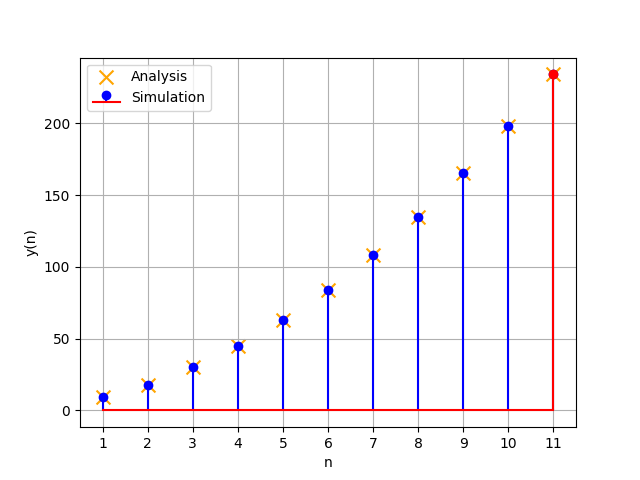
\includegraphics[width = \columnwidth]{figs/fig2}
		\caption{y(n) vs n}
		\centering
		\label{fig: fig2}
	\end{figure}
\end{document}